%Packages and classes

\documentclass{ou-thesis}

%\usepackage{epsfig}
\usepackage{graphics}
\usepackage{amsmath}
\usepackage{rotating}
\usepackage[english]{babel}
\usepackage{morefloats}
\usepackage{todonotes}
\usepackage{chemformula}
\usepackage{pdfpages}
\usepackage{float}
\usepackage{listings}

\renewcommand{\floatpagefraction}{1}



\newtheorem{theorem}{Theorem}
\setcounter{page}{1} \pagenumbering{arabic}
\ifpdf
    \pdfinfo {
      /Title (HABs)
      /Subject (Environmental Science)
      /Author (Hamzah D. Ansari)
      /Keywords (HABs)
   }
\fi




\makeatletter




\begin{document}

\graphicspath{{./figures/}}
\title{Predictive Modeling of Harmful Algal Blooms}
\author{Hamzah D. Ansari}
\degree{Master of Science in}
\department{Chemistry}
\degreeyear{2018}
\chairperson{Roman Dembinski}
\committeetwo{Linda Schweitzer}
\committeeone{David C. Szlag}
\committeethree{Thomas Raffel}
\dedication{I dedicate my thesis to my best friends and my beloved family for providing me love and support through my graduate program. I also dedicate this thesis to Carl Sagan who instill my curiosity and pursuit of scienctific knowledge.}
\acknowledgmentfile{Acknowledgment}
\abstractfile{Abstract}

\makefrontmatter


\renewcommand{\bibname}{REFERENCES}

\chapter{INTRODUCTION}
% this is needed but save this, it was in the template.
  \setlength{\parindent}{.5 in}
   \raggedright\setlength{\parindent}{.5 in}

Around the world, cyanobacteria and algae can grow rapidly, killing aquatic life and painting coastal beaches bright green. The rapid growth of cyanobacteria and algae threatens the ecosystem. Harmful Algal Blooms (HABs) is a phenomenon where cyanobacteria and algae grows rapidly, dominating with large biomass and often paints the surface of any waterbody bright green. The large biomass of HABs greatly stresses the aquatic ecosystem. The increasing occurence is a major concern, threatening the Luastrine Great Lakes \cite{raikow_dominance_2004}. Recently, HABs affected over 400,000 people hindering drinking water supply in Toledo, Ohio preventing the citizens to drink or bath from their homes \cite{mann_toledo_2014}.


One of Michigan's greatest assets is the bountiful amount of inland lakes. Much of the inland lakes provides beautiful shoreline property and great real estate. The attractive features provides us with a multitude of recreational activities. For certain areas, recreational tourism drives much of the economics for small towns. HABs greatly diminishes the quality of this feature. Lakes that are painted green from HABs transforms this beauty into an ugly mess. One of the most arguable reasons to address the health of the inland lakes is its role in providing life within an ecosystem.  Freshwater is without a doubt an vital resource for all living organisms, and the blight from HABs destroys our water sources.

\section{Harmful Algal Blooms}


Cyanobacteria, as one of the oldest living organism had influenced much of the Earth's history. Cyanobacteria are a highly resilient gram-negative prokaryote which uses photosynthesis for its energy source \cite{rastogi_cyanotoxin-microcystins:_2014}. As one of the oldest prokaryotic organism, there are evidence of their existence 2.5 billion years ago \cite{paerl_moving_2016}. As a primary producer, cyanobacteria has provided much of the Earth's oxygen between 2.45 and 2.32 Ga known as the Great Oxidation Event\cite{farquhar_geological_2011}. Blooms are diverse rainging from multiple organisms.  from cyanobacteria, diatoms, algae, dinoflagellates,  rainging from  occure worldwide.  .Currently cyanobacteria and algae is vital as it fixate a large amount of CO2 from their environment \cite{van_mooy_quorum_2012}.

However, as the population grows exceeding the capacity of the environment, they become dangerous.
In most cases they naturally occuring cyanobacteria and algae harmless, coexisting with the environment and an important primary producer for an ecosystem. However, when growth becomes too excessively it becomes a major issue. Some species of cyanobacteria produces a variety of toxins. HABs often impare water quality and become poisenous, threatening life of fauna \cite{martins_seasonal_2011}. Animals drinking impaired water can propogate toxins  \cite{koreiviene_cyanotoxin_2014}.  Exposure through dermal contact can be an irritant, and ingestion results with acute toxicity eventually leading to liver failure. HABs can create lipopolysaccharide which are endotoxic and create rashs on human skin when exposed \cite{moore_richard_cyanobacterial_1993}. Ingestion of microcystin by directly drinking water from an affected lake could  lead to liver failure and eventually causing death \cite{monks_potent_2007}. In recent years, increasing anthropological activities may have increased the occurance of HABs \cite{paerl_controlling_2011}. HABs is believed to be caused mostly by agricultural runnoff and catalyzed by impervious surfaces \cite{smith_eutrophication_2009}.

HABs are dangerous ecologically and harmful to human health. Swimming in any waterbody with an excessive growth of cyanobacteria is a risk. HABs will most likely have a variety of toxins with a ranging amount of symptoms from dermal irritants, hepatoxicity, possibly leading to cancer \cite{paerl_controlling_2011}. Many of the species that are producing hepatoxins and neurotoxins in high amounts are killing livestock and wildlife \cite{anderson_harmful_2002}.The harm caused by HABs does not neccessarily come from the toxins itself. HABs can be present with visible blooms but with no toxins present. Even with no toxins present in waterbodies, there are still implications that are still dangerous. The rapid biomass of leads to a layer of scum which depletes oxygen as the dead cells are consumed by other microorganisms \cite{anderson_harmful_2002}. Hypoxia essentially stops all respiration for any living organisms. Lake Erie faced this issue where massive amounts of fish died off due to depleted oxygen which vastly affected the condition of the lake \cite{charlton_oxygen_1980}.

They are utilized in positive ways, from providing nutritious supplements and producing energy. Some genera such as \emph{Spirulina} and \emph{Chlorella} are used as dietary supplemnts, providing an alternative source of omega-3 and omega-6 fatty acids, aimly for vegetarians \cite{guevara-gonzalez_microalgae_2014}. Although using as supplments can be dangerous as studies shows some have contain toxins such as nodularin and microcystin \cite{turner_development_2018}. The concern has brought much attention, as businessess are now employing a quality control screening for detecting any toxins in their products \cite{manali_detection_2017}. Algal biomass are being investigated for being used as biofuels as it produces heavy oils \cite{demirbas_use_2010}.

WORK

State government and health officials continuously monitor and analyze surface and drinking water for microcystin. The World Health Organization (WHO) have guidance level of 1 $\mu$g/mL for drinking water \cite{world_health_organization_guidelines_2003} For the state of Michigan, microcystin guidance level for recreational surface water are 4 $\mu$g/mL \cite{us_epa_draft_2016}. Levels above those guidelines requires state officials to issue warnings not to swim in the effected area. The emerging issues from HABs are becoming more problematic for drinking water and recreational use, which needs to be monitored. There are many methods of analysis for detection of either cyanobacteria or the toxins. The current routine methods employed by state agencies are ELISA kits by Abraxxis . This is an antibody method that measures the ADDA-moiety of the microcystin. Analytical protocols currently employed are quasi reliable but may fail to detect HABs on the early onset.

WORK



\section{Goals and Aims}

In our survey, we focused on microcystins (MC), a cyclic hepatoxin which prevalent in Michigan’s inland lakes. MC’s in particular are a threat to human health in recreational waters and  most importantly, endanger drinking water sources.

My goal is to explore what drives HABs. Previous studies have built models based on variables that we have collected. With the collected observations, I investigated the best possible predictive model from our dataset. Microcystin concentrations from LC-MS/MS results will be the response variable. Independent varialbles are from land use, lake limnology, \emph{chlorophyll-a}, \emph{phycocyanin}, amount of \emph{Dreissena polymorpha}, dissolved nutrients. The goal is to have a model that is simple and is robust.



\section{Objectives}









\chapter{LITERATURE REVIEW}



\section{Cyanotoxins}

Cyanobacterial toxins are vastly diverse and is continuously being discovered. More than 600 peptides have been discovered and still discovering more \cite{welker_cyanobacterial_2006}. They create a variety of toxins with a range of different mechanism of toxicity. Black Band Disease caused by a thick and dark filamentous cyanobacteria have poisoned coral reafs and out-compete against other organisms \cite{meyer_microbiome_2015}

Saxitoxin are sodium channel blockers \cite{moore_richard_cyanobacterial_1993}


A study found microcystin presists within the cell and does not break down intracellular by metabolic process \cite{rohrlack_fate_2007}




The structure of microcystin is composed of D-erythro$\beta$-methylaspatric acid (D-MeAsp), 3-amino-9-methoxy-10-phenyl-2,6,8-trimethyl-deca-4,6-dienoic acid (Adda), \textit{N}-methyldehydro-alanine (Mdha) and other variable amino acids \cite{nishizawa_genetic_1999}.
Microcystins are produced by a mix of to systems, polyketide synthase(PKS) and nonribosomal peptide synthetase (NRPS) \cite{tillett_structural_2000}.
The genetic mechanism of microcystin synthisis involves multiple protien modules which are responsible for incorporating different amino acids, utlimatly creating the cyclic peptide \cite{nishizawa_genetic_1999}. The underlying mechanism involves with activating adenlylation and peptite elongation by thioesterase domains \cite{welker_cyanobacterial_2006}.
Nearly all cyanobacteria contain thioesterase domains \cite{tonk_production_2009}. Microcystin have various forms due to different L$-$ammino acids.
There are over 100 known variation of microcystin with 6 congeners recognized by the EPA are MC-LR, MC-RR and MC-LA \cite{puddick_modulation_2016}. The most frequently occurent congener variant is MC-LR \cite{rastogi_cyanotoxin-microcystins:_2014}. Figure \ref{structure1} shows the structure of MC-LR which contains L-luecine (L) and L-Arginine (R). Other amino acids such as


\begin{figure}[t]
  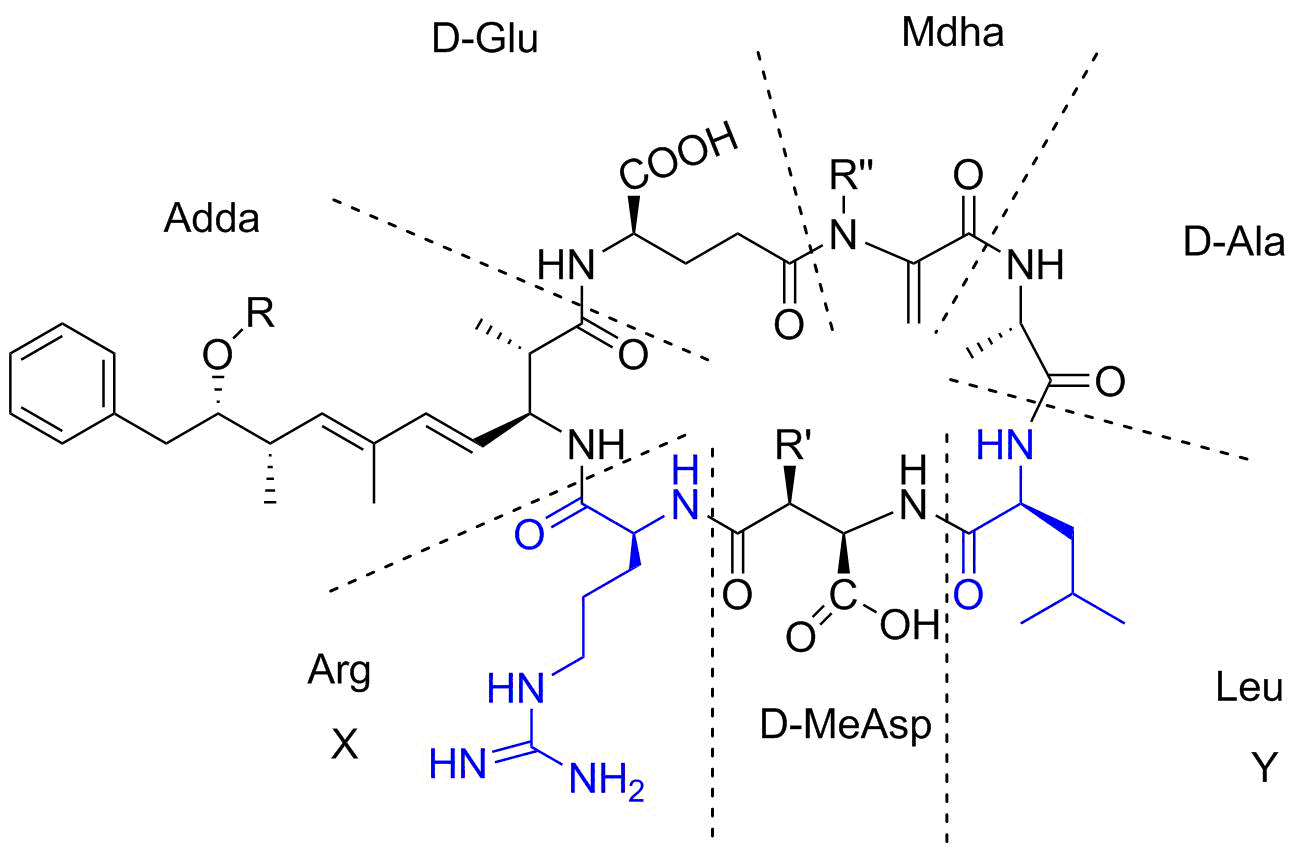
\includegraphics[width=\textwidth]{Microcystin-LR.eps}
  \caption{Structure of Microcystin-LR}
  General structure of Microcystin-LR. a) Adda group responsible for the hepatoxicity
  b) L-leucine, a variable amino group amongst other congeners.
  c) L-argineneVariable amino group.
  \label{structure1}
\end{figure}


\section{Environmental Drivers}

Understanding the energy source for cyanobacteria is vital to predict what drives HABs occurences. Cyanobacteria can fixate carbon from \ch{CO2}

Nutritional elements from organic and inorganic forms provide food. In certain circumstances, nutrients such as inorganic nitrogen or phosphorus are limiting growth factors.

Phosphorus is commonly used in bacteria for making their cell walls. Co-polymers with majority of their bonds consisting of phosphodiaster bonds.


A study by Korea Research Institute of Bioscience and Biotechnology found 3-week lagged water temprature to be one of the best predictor variable in their model search \cite{ahn_evaluation_2011}. They found total nitrogen having a negative effect, which is they do not expecte \cite{ahn_evaluation_2011}.


There are many possible sources of nutrients that can contribute the growth of cyanobacteria and algae. The frequency of HABs around the world have increased, most likely due to the rise of anthropogenic effects such as farming, waste management, and non-point source pollution. \cite{wilhelm_relationships_2011}.
Sources from sewage from septic tanks, animal waste and agricultural runnoff  could contribute to HABs. Nutrients from agriculture runnoff can have a great effect as fertilizer application has been increasing \cite{anderson_harmful_2002}.

Cyanobacteria have a unique way of aquiring nutrients under extreme conditions. They can utilize a process called quorom sensing which they coordinate with eachother by using a signling hormone acylated homoserine lactones \cite{van_mooy_quorum_2012}.















\chapter{SURVEY METHODS AND DESIGN}

For the summer of 2017 a total of 29 inland lakes were sampled.  Prior to sampling, permission of riparian owner was obtained for most lakes. Sample surveying began on the month of June 2017 until October 2017. Each month every lake one was sampled once. Sampling location was chosen by ease of access or on the property of established riparian owners. See table \ref{table:Surveyed Lakes} for the list of sampled lake and their location.

\section{Water Sampling}



\begin{table}
\caption{List of Surveyed Lakes}
\label{table:Surveyed Lakes}
\begin{center}
\scalebox{0.8}{
\begin{tabular}{|l|l|l|r|r|l|}
\hline
\multicolumn{1}{|c|}{Name of Lake} & \multicolumn{1}{c|}{Shorten Code} & \multicolumn{1}{c|}{County} & \multicolumn{1}{c|}{Longitude} & \multicolumn{1}{c|}{Latitude} & \multicolumn{1}{c|}{HUC 14 Reachcode} \\ \hline
Bear Lake & BEA & Kalkaska & -84.9438079727 & 44.7286139551 & 04060103001048 \\ \hline
Belleville Lake & BEL & Wayne & -83.4663770506 & 42.2145253455 & 04090005001822 \\ \hline
Bogie Lake & BOG & Oakland & -83.5054334514 & 42.6188513679 & 04090005001348 \\ \hline
Brighton Lake & BRI & Livingston & -83.7958137995 & 42.5169054061 & 04090005001500 \\ \hline
Coldwater Lake & COL & Isabella & -84.9565922285 & 43.6613607551 & 04080202000902 \\ \hline
Deer Lake & DEE & Charlevoix & -84.9770123186 & 45.166441811 & 04060105001116 \\ \hline
Ford Lake & FOR & Washtenaw & -83.5849122567 & 42.2159133043 & 04090005001823 \\ \hline
Houghton Lake & HOU & Roscommon & -84.7262816343 & 44.3385407778 & 04060102002461 \\ \hline
Hudson Lake & HUD & Lenawee & -84.2545514803 & 41.835000535 & 04100002001317 \\ \hline
Intermediate lake & INT & Antrim & -85.2293359783 & 45.0265435299 & 04060105003435 \\ \hline
Lake Cadillac & CAD & Wexford & -85.4266252378 & 44.2410192547 & 04060102001951 \\ \hline
Lake Margrethe & MAR & Crawford & -84.7830175986 & 44.6464747348 & 04060103001058 \\ \hline
Lake Nepessing & NEP & Lapeer & -83.3728265865 & 43.0161554865 & 04080204001601 \\ \hline
Lime Lake & LIM & Hillsdale & -84.3791188315 & 41.7861576065 & 04100006000872 \\ \hline
Little Glen Lake & LGL & Leelanac & -85.963633169 & 44.8687577197 & 04060104000456 \\ \hline
Little Round Lake & LRO & Lenawee & -84.3527742524 & 41.9093334799 & 04100006000858 \\ \hline
Manitou Lake & MAN & Shiawassee & -84.2038069227 & 42.925537136 & 04050005000939 \\ \hline
Ore Lake & ORE & Livingston & -83.7959940227 & 42.4805569493 & 04090005001574 \\ \hline
Paradise Lake & PAR & Emmett & -84.7512093045 & 45.6872890124 & 04060105001063 \\ \hline
Platte Lake & PLA & Benzie & -86.092789204 & 44.6900468421 & 04060104000558 \\ \hline
Pontiac Lake & PON & Oakland & -83.451096479 & 42.6664394508 & 04090005001288 \\ \hline
Posey lake & POS & Lenawee & -84.3007962072 & 41.8970465491 & 04100006000857 \\ \hline
Round Lake & ROU & Lenawee & -84.1318219224 & 42.0712488438 & 04100002001130 \\ \hline
Sanford Lake & SAN & Midland & -84.3860517762 & 43.7104273774 & 04080201001468 \\ \hline
Silver Lake & SIL & Grand Traverse & -85.687150728 & 44.6980286859 & 04060105003542 \\ \hline
Stony Creek Lake & STO & Oakland & -83.0870627175 & 42.7260717429 & 04090003001029 \\ \hline
Sugden Lake & SUG & Oakland & -83.4972563639 & 42.6173106359 & 04090005001347 \\ \hline
West Twin Lake & WTL & Montmorency & -84.3501403918 & 44.8762035424 & 04070007001271 \\ \hline
Wixom Lake & WIX & Gladwin & -84.3537506311 & 43.8276751177 & 04080201001442 \\ \hline
\end{tabular}}
\end{center}
\end{table}




\section{Analysis Method}

\subsection{ELISA}

A commercial Microcystins/Nodularins ADDA ELISA kit from Abraxis was used to analyze microcystin concentrations. For cell lysis, all samples were put through 3 freeze-thaw cycles.  Each cycle consisted of freezing the bottles in a -20 C freezer until complete solidity and then thawing in a 37 C water bath until completely melted. Samples were mixed by inversion and placed in the refrigerator until needed for the assay.

Analysis based on the assay standard curve was done using EPA method 546. The ELISA standards include 0, 0.15, 0.4, 1, 2, and 5 ppb. The standard curve was created using a 4-parameter regression as used in EPA method 546. The regression from the assay produced and $R^2$ of 0.997. According to Method 546 an acceptable R2 is greater than 0.98.  Coefficients of variation (CV) for all replicate standards were below 10 accept for the 5 ppb which is acceptable. Two continuing calibration verification controls were used with the assay and were within the expected variation. The 0.75 ppb was reporting at 0.719 ppb which is within the inherent $\pm$ 0.185 ppb range. The low 0.4 ppb standard reported at 0.336 ppb which is within the  0.16 ppb range of the standard. In all our analysis none were invalidated as CV $> 15\%$  indicated in the EPA method. The percent CV was calculated using the quotient of the absorbance standard deviation and the average absorbance then multiplying by 100.

Three field blanks were ran and were below the reportable limit. Some samples with high concentrations were diluted 1:10 prior to analysis. Brighton, Hudson, and Wixom throughout all of the analysis had notable concentrations above the detection limit of 5ppb.

\subsection{LC-MS/MS}

A 3.5 ml aliquot of each sample prepared for the ADDA-ELISA analyses described above was transferred to glass vials suitable for the Thermo Scientific EQuan MAX (online sample concentrator).  These sample were transported to Wayne State University (WSU) and analyzed for 12 microcystin congeners, and nodularin.  The Westrick group at the WSU Lumigen Instrument Center (LIC) has developed a high-throughput LC-MS/MS analysis for microcystins in surface and drinking water analyses. The Westrick group’s LC-MS/MS platform includes a Thermo Scientific EQuan MAX (online sample concentrator) and ThermoFisher’s UltiMate 3000 (UHPLC) system and a TSQ Quantiva (MS/MS). The microcystin on-line concentration method is validated for 12 microcystins.  \ref{spectra} shows a standard chromatogram of all 12 microcystins, nodularin, and the deuterated internal standard (C2D5 MCY-LR) eluting between 2.2 – 5.2 minutes allowing for the total analyses time to be less than 12 minutes.  Detection limits are 0.03 ppb for microcystins.

\begin{figure}[h]
  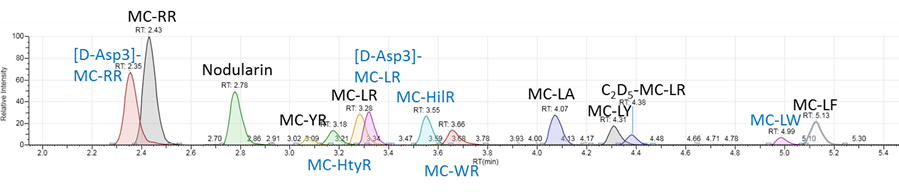
\includegraphics{LCMS_CONGENERS}
  \caption{Liquid chromotography-mass spectrometry chromatogram of the microcystin congeners}
  \label{spectra}
\end{figure}

\subsection{Nutrients}


Three distinct nutrient grab samples were sampled at each lake. Two 125-mL HPDE Nalgene bottles were used to collect acid-preserved water samples with 2mL of 3M H2SO4, resulting to pH < 2. One will be analyzed for ammonia-N and nitrate+nitrite-N by our lab at Oakland University and the other is allocated for total phosphorus and total nitrogen run by Lake Superior State University. One 50-mL conical tube was used to collect ambient water sample for ortho-phosphate analysis. Samples were kept cool at 4C during transport and stored at -20C. Upon receiving samples from field samplers samples are thawed if frozen and kept cool at 4C. All lake water samples are homogenized by inverting 8 times and aliquoted into 15 mL vials. Next the water samples are transfered to 15-mL centrifuge vials and centrifuged at 3000rpm for 45 seconds. The supernatant was collected into a clean 3 mL vial and analyzed by AQ1 auto sampler. Ammonia-N is analyzed by an equivalent EPA method (USEPA 600/R-93/100 Method 350.1, Revision 2.0).

Calibration curves are generated with day of analysis. Standards for each analysis were prepared fresh for each batch of samples. The solids of each standard is hygroscopic. Solid standards are incubated at 40C then cooled in a sealed glass desiccator prior to measuring required mass. Once mass of standards are stable between incubation and cooling we proceded creating standard solutions. Standard solutions are diluted with milli-Q water to the appropriate concentrations and pH buffered to match acid preservation. For each nutrient analysis, the highest concentration of the range is loaded unto the AQ1 auto-sampler along with the appropriate diluent. The auto-sampler automatically dilute 6 concentrations points and generates the standard curves. Diluent for nitrate+nitrite and ammonia calibration curve is pH buffered milli-Q water. Ortho-phosphate uses milli-Q water as the diluent.

Constant Control Variable (CCV), and Constant Control Blanks (CCB) were analyzed between every 10 sample or less runs. CCVs are prepared along with standards prior to analysis. The concentrations for ortho-phosphate, nitrate+nitrite and ammonia are 0.100 mg P/L, 1.50 mg N/L, and 0.500 mg N/L respectively. Upon every batch of samples, method blanks are also processed during centrifuge steps. CCBs are prepared by analyzing our milli-Q water source and the method blanks. CCV's were within 10\% range of actual concentration. CCB's were all no higher than the mininum detection limit. Throughout each analysis, few selected lakes were spiked with known concentration of analyte and analyzed for spike recovery. A total of 36 spike recovery analysis was run. Ammonia and nitrate+nitrite had excellent recovery, averaging  86\% and 94\%. Ortho-phosphate had poor recovery, averaging at 60\%.

Each sampling month, field duplicates and field blanks were also collected and analyzed. Relative percent difference of field duplicated were mostly low. In the instance of high percent difference above 25, the measured values were relatively low except for one sample in Wixom lake in September. Field blanks were also low except for Ammonia results in July and August.


\subsection{QPCR}

Each lake, 100mL of water sample was collected in a sterile IDEXX vessel. Samples were collected by wading until water height reached waist height and taken roughly one foot below water surface.Sampled lakes close to Oakland University were  transported at 4-6C back to Oakland University for water filteration. Remote sampled sites are filtered on site with portable Santino pump and stored at -20C until sampling route is back. Water samples are filtered through 3  m pore sized polycarbonate filter and transferred into BioGX \todo{citation} vials. BioGX vials are stored at -80C until analysis. BioGx vials contains 500 uL of lysis buffer, lysis beads and filtrate. For cell lysis, vials were virously shaken by bead beater for 2 minutes. After bead beaten, sample vials were centrifuged for 1 min. Supernatent was transferred to a microcentrifuge tube and centrifuged for 5 min, then transferred the final supernatent to another set of microcentrifuge tubes for PCR template.  Sample extracts are stored at 4C and analyzed within the day.

Phytoxigene CyanoDtec test was preformed with Applied Biosystem StepOnePlus PCR. Total Cyanobacteria 16s rRNA and toxin gene assay were analyzed in parallel for each month of grab samples. Prior to setting up PCR template, lyophilised mastermix reconstituted with PCR-Grade water. The PCR reaction mix contained 5 ul of template/sample extracts and 20 ul of rehydrated mastermix.  Each sample were run in singlicate. Positive standards for target genes  were run on each PCR analysis. CyanoNAS nucleic standards are removed from -20C and allowed to thaw prior to analysis.  Standards were run in duplicate.

PCR heat cycles were programmed with initial denaturing step at 95C for 2 min, then a repeat of 95C for 15 seconds and 60C for 30 seconds reaching a total of 40 cycles. The appropriate gene targets filters were set to match the emission spectra of each probes. Each PCR run, standard curve is generated  from within the StepOnePlus software. CT threshold and baseline was manually assigned for each run by visually assessing each target run. The calculated gene copies are done automatically by the StepOnePlus software, expressed in Gene Copies/$\mu$L of lysate. The final reportable value is given by this equation:

\begin{center}
  $Genecopies/mL = (Genecopies/\mu L of lysate) \times (\frac{500\mu L of lysate}{\text{mL of Sample Volume}})$
\end{center}




\section{Geographic Information System (GIS)}

Watershed delineation and calculation of land use was done using quantum geographic information system (QGIS) \cite{qgis_development_team_qgis_2009}. Elevation data was downloaded in bulk by an FTP client. Elevation mosaic raster files for the state of Michigan was downloaded from Natural Resources Conservation Services
%%%
nder Spatial Analysis Tools the “Fill” tool was applied to the DEM to remove any sinks, thus creating a filled DEM. Next the “Flow Direction” tool is used with the filled DEM as the input. This results a flow direction grid using D8 algorithm. Next is to create a flow accumulation grid with “Flow Accumulation” tool using the flow direction raster as the input. This calculates the flow by the number of cells that accumulates into each cell. With the flow accumulation raster, any value greater than 4000 is colored to visualize the main flowlines. This aids in selecting the pour points for each of the selected lakes. A new feature class is created and manually created pour points for each lake. Using the visualized flow stream, the pour point is determined where flow accumulation is highest within the perimeter of the lake. The feature class is then rasterized by the tool “Snap Pour Point” with the snap distance parameter set to 10 meters. The watershed is delineated with the pour points and flow direction raster. Finally, the watershed raster is then converted into a polygon with the “Raster to Polygon” conversion tool


The land use raster is reclassified into anderson level-II categories using “Reclassify” tool. See table 1 for the details of classification. The land use counts of cells is calculated by using “Tabulate Area” tool. Using the field calculator, the percentage of land use is populated and exported for statistical analysis in Program R

\section{Statistical Analysis}



\chapter{RESULTS}

\section{Summary}



\begin{table}[!ht]
  \label{variable}
  \caption{Variable Shorten Name and Transformation Summary}
\centering
\scalebox{0.6}{
\begin{tabular}{lll}
  \hline
Short Name & Variable Name (Units) & Transformation \\
  \hline
OP & Ortho-P (mg-P/L) & log10(OP + 0.003) \\
  NOX & Nitrate/Nitrite (mg-N/L) & log10(NOX + 0.04) \\
  NH3 & Ammonia (mg-N/L) & log10(NH3 + 0.006) \\
  TP & Total phosphorus (mg-P/L) & log10(TP + 0.002) \\
  TKN & Total kjeldahl nitrogen (mg-N/L) & log10(TKN + 0.07) \\
  TNTP & Total nitrogen to total phosphorus ratio & None \\
  X16SRNA & Cyano 16s rRNA gene copies (cp/mL) & log10(X16SRNA + 20) \\
  MCYE & mcyE gene copies (cp/mL) & log10(MCYE + 20) \\
  SUM & Microcysin sum from all 12 MC congeners (ppb) & log10(SUM + 0.03) \\
  wtemp & Water temprature at time of sampling (Celcius) & None \\
  pH & pH & None \\
  do & Dissolved oxygen (mg/L) & log10(do + 0.01) \\
  conduc & Conductance (uS/cm) & log10(conduc + 0.01) \\
  turb & Turbidity (NTU) & log10(turb + 0.01) \\
  chloro & Chloraphyll-a (RFU) & log10(chloro + 0.01) \\
  phyco & Phycocyanin (RFU) & log10(phyco + 0.01) \\
  TN & Total nitrogen (mg-N/L) & log10(TN + 0.116) \\
  Max\_Depth & Maximum depth of lake (meters) & None \\
  Lake\_Area\_sqKm & Lake area (sq Km) & log10(Lake\_Area\_sqKm + 1) \\
  Watershed\_Area\_sqKm & Watershed Area (sq Km) & log10(Watershed\_Area\_sqKm + 1) \\
  Lake Area\_Watershed Ratio & Lake area to watershed area ratio & log10(Lake Area\_Watershed Ratio + 1) \\
  Water & Land-Use percentage in lakes watershed & None \\
  Developed & Land-Use percentage in lakess watershed & None \\
  Barren & Land-Use percentage in lakes watershed & None \\
  Forest & Land-Use percentage in lakes watershed & None \\
  Shrubs & Land-Use percentage in lakes watershed & None \\
  Herbaceous & Land-Use percentage in lakes watershed & None \\
  Agriculture & Land-Use percentage in lakes watershed & None \\
  Wetlands & Land-Use percentage in lakes watershed & None \\
  LogMusselMass & Zebra mussel Mass (grams) & log10(MusselMass + 1) \\
  LogMusselNum & Zebra mussel counts & log10(MusselNum + 1) \\
  precip3 & Average precipitation 3 days before sampling  (mm) & log10(precip3 + 1) \\
  temp3ambient & Average temperature 3 days before sampling (Celcius) & None \\
  precip5 & Average precipitation 5 days before sampling (mm) & log10(precip5 + 1) \\
  temp5ambient & Average temperature 5 days before sampling (Celcius) & None \\
  precip7 & Average precipitation 7 days before sampling (mm) & log10(precip7 + 1) \\
  temp7ambient & Average temperature 7 days before sampling (Celcius) & None \\
  precip30 & Average precipitation 30 days before sampling (mm) & log10(precip30 + 1) \\
  temp30ambinet & Average temperature 30 days before sampling(Celcius) & None \\
  hobotemp & Average Temprature from Hobo pendant one month before sampling (Celcius) & None \\
  hobolight & Average light intensity from Hobo pendant one month before sampling (lux) & log10(hobolight +1) \\
   \hline
\end{tabular}}
\end{table}




\section{Hypothesis Test}



\section{Predictive Modeling}

\subsection{Feature Selection}

From our collected dataset, we assessed each variable's distribution and log-transformed to fit a normal distribution. To solve the problem of data values = 0, we added the corresponding mininum detection limit first, then applied a log trasformation. See table \ref{variable} for which variable was transformed and the shorten variable name.

Canidate variables will be selected from best subset regression. Subset analysis is done on an averaged dataset based on each lake. Measurements from each lake is a factor that may contribute as a random effect. The averaged data solves an issue where measurements from each lake is pseudoreplicated, as suggested by C. Eisenhart \cite{eisenhart_assumptions_1947}. This results with  $N=29$ observations. The averaged data is then log transformed as described in table \ref{variable}. From our best subset analysis, we observed mcyE, turbidity, max depth of the lake (see figure \ref{subset}).

With the best variables from the regression subset, a forward and backward step-wise regression will be preformed to further search the best fit model. First, variables will be backwardly selected based on Anova type II Sum of Square test. Type II  SS tests each variable after accounting all the other variable.


Our best model will be chosen by the lowest Bayesian Information Criterion (BIC).


\begin{figure}[!t]
  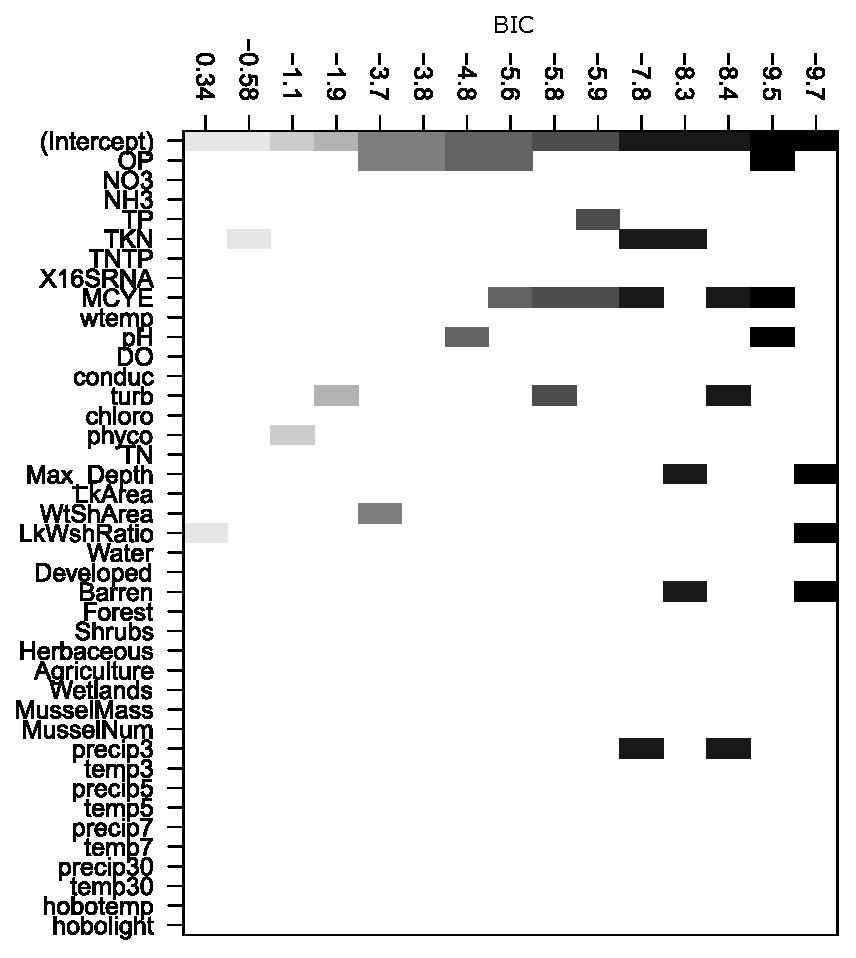
\includegraphics[scale=0.8]{Subset}
  \caption{Best Subset Regression}
  \label{subset}
  Each row is a model, if a variable is included in the model it is represented as a shaded rectangle. The BIC is plotted on the y axis where the lowest value is higher up on the axis. The better the model, the lower the BIC, thus the top rows are the better model.
\end{figure}






\subsection{Linear Mixed Model}








\chapter{DISCUSSIONS}

Prior to our survey, we hypothesized if the lake's watershed is predominantly urbanized areas, then we would expect the increase probability of microcystin concentrations. The excessive growth of cyanobacteria increase the likelihood of microcystin production. Nutrients increase the trophic conditions which drives the growth of cyanobacteria, which could increase the probability of microcystins. Developed/urban and agriculture areas may have an influence on nutrients because of more possible sources like applied fertilizer or leaky septic tanks. Impervious surface area withing the lake's watershed may also have a possible influence nutrient mobility, which may also drive microcystin production.




\clearpage
\newpage

\bibliographystyle{achemso}
\bibliography{sources}

\begin{appendix}

\appendixchapter{Exploratory Analysis and Summary Statistics}






\newpage


\begin{figure}[!t]
  \caption{Correlation Matrix}
  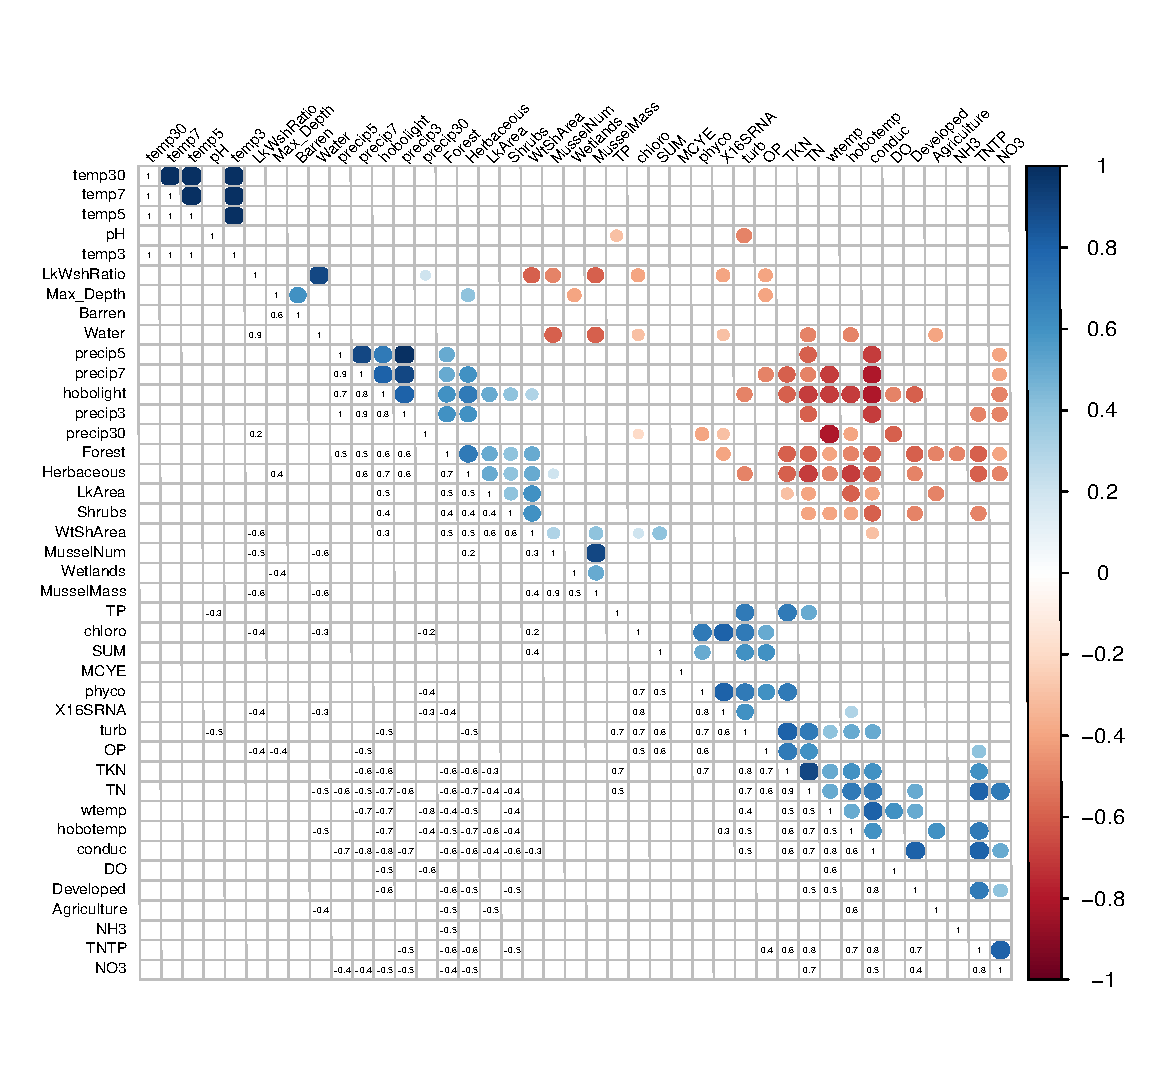
\includegraphics{matrix}
  Positive correlation is represented with solid blue box and negative correlation with scored box.
  \label{matrix}
\end{figure}

\begin{figure}[t]
  \caption{}
  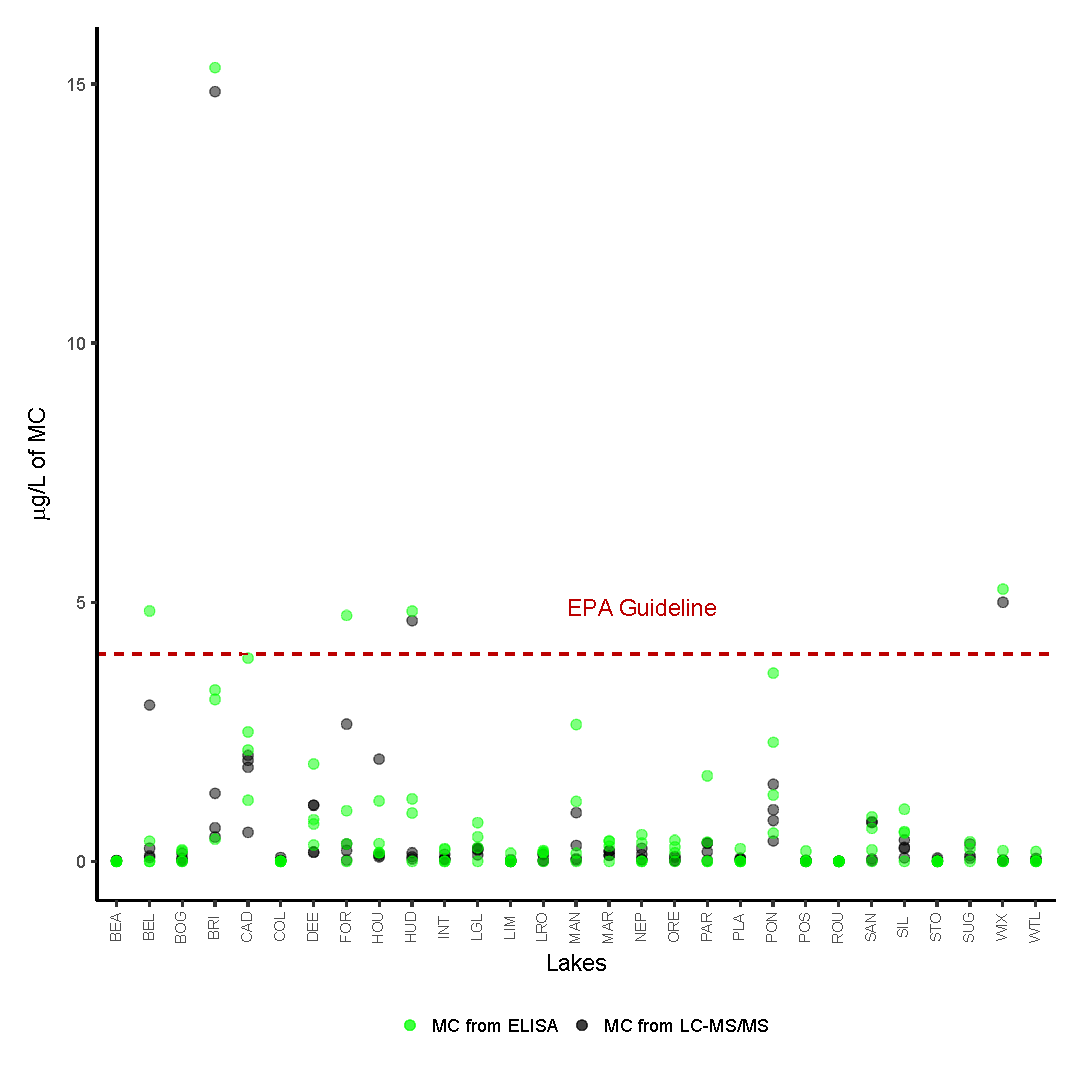
\includegraphics[height=10cm, width=12cm]{Microcystin}
  \label{Yesa}
\end{figure}

\newpage














\newpage


\begin{table}[!htbp]
  \centering
  \caption{QPCR}
  \label{QPCR}
  \begin{tabular}{@{\extracolsep{5pt}}lccccc}
  \\[-1.8ex]\hline
  \hline \\[-1.8ex]
  Statistic & \multicolumn{1}{c}{N} & \multicolumn{1}{c}{Mean} & \multicolumn{1}{c}{St. Dev.} & \multicolumn{1}{c}{Min} & \multicolumn{1}{c}{Max} \\
  \hline \\[-1.8ex]
  16S rRNA & 112 & 405,761 & 798,946 & 0 & 6,765,631 \\
  mcyE & 91 & 8,517 & 49,396 & 0 & 467,174 \\
  cyrA & 93 & 0 & 0 & 0 & 0 \\
  sxtA & 93 & 0 & 0 & 0 & 0 \\
  \hline \\[-1.8ex]
  \multicolumn{6}{r}{* Values are expressed as Gene copies/$\mu$L} \\
  \end{tabular}
  \end{table}

\newpage


\begin{table}[!htbp]
  \centering
  \caption{}
  \label{}
\begin{tabular}{@{\extracolsep{5pt}}lccccc}
\\[-1.8ex]\hline
\hline \\[-1.8ex]
Statistic & \multicolumn{1}{c}{N} & \multicolumn{1}{c}{Mean} & \multicolumn{1}{c}{St. Dev.} & \multicolumn{1}{c}{Min} & \multicolumn{1}{c}{Max} \\
\hline \\[-1.8ex]
 Orthophosphate (mg P/L) & 114 & 0.015 & 0.030 & 0.000 & 0.237 \\
Nitrate+Nitrite (mg N/L) & 115 & 0.199 & 0.443 & 0.000 & 2.827 \\
Ammonia (mg N/L)  & 115 & 0.112 & 0.281 & 0.000 & 2.338 \\
Total Phosphorus (mg P/L) & 114 & 0.055 & 0.037 & 0.000 & 0.239 \\
Total Kjeldahl Nitrogen (mg N/L) & 114 & 0.763 & 0.602 & 0.000 & 4.555 \\
Total Nitrogen & 114 & 1.074 & 0.870 & 0.103 & 4.717 \\
\hline \\[-1.8ex]
\end{tabular}
\end{table}


\newpage

\begin{table}[!t]
\centering
\caption{AQ1 QAQC}
\label{AQ1 Quality Control}
\begin{tabular}{llllll}
  \hline
Date     & Analysis        & R2     & Slope & Intercept & \%Carryover \\
  \hline
20170707 & Orthophosphate     & 0.9993 & 2.61  & 0.00      & 0.20        \\
20170807 & Orthophosphate     & 0.9993 & 2.43  & 0.00      & 0.20        \\
20170909 & Orthophosphate     & 0.9996 & 2.94  & -0.01     & 0.20        \\
20170711 & Nitrate+Nitrite & 1.0000 & 16.49 & -0.51     & 0.10        \\
20170814 & Nitrate+Nitrite & 0.9990 & 18.50 & -0.43     & 0.20        \\
20170808 & Nitrate+Nitrite & 1.0000 & 16.57 & -0.47     & 0.40        \\
20170913 & Nitrate+Nitrite & 0.9997 & 17.72 & -0.53     & 0.90        \\
20170711 & Ammonia         & 0.9996 & 1.63  & -0.29     & 0.90        \\
20170809 & Ammonia         & 0.9998 & 1.70  & -0.20     & 1.80        \\
20170817 & Ammonia         & 0.9995 & 1.59  & -0.33     & 0.30        \\
20170912 & Ammonia         & 0.9996 & 1.67  & -0.09     & 0.70        \\
20170913 & Ammonia         & 0.9996 & 1.67  & -0.09     & 0.70
\end{tabular}
\end{table}

\newpage

\appendixchapter{Lake Information}


\appendixchapter{Analysis of MC}

\section*{Analysis of MC Data}

\indent Analysis of MC is complicated by the large number of variants or congeners.  LC-MS/MS quantitative analysis is limited to known congeners with commercial sources.  The Adda ELISA is not congener independent.

To test our hypothesis that the discrepancy between the ELISA and LC-MS/MS we log transformed the data and calculated the difference between the methods, creating a dependent variable, delta.  The censored values used 0.15 ppb for the ELISA and 0.03 ppb for all MC congeners.  A correlation matix was prepared using the package R

\newpage

\begin{figure}[!htp]
  \caption{}
  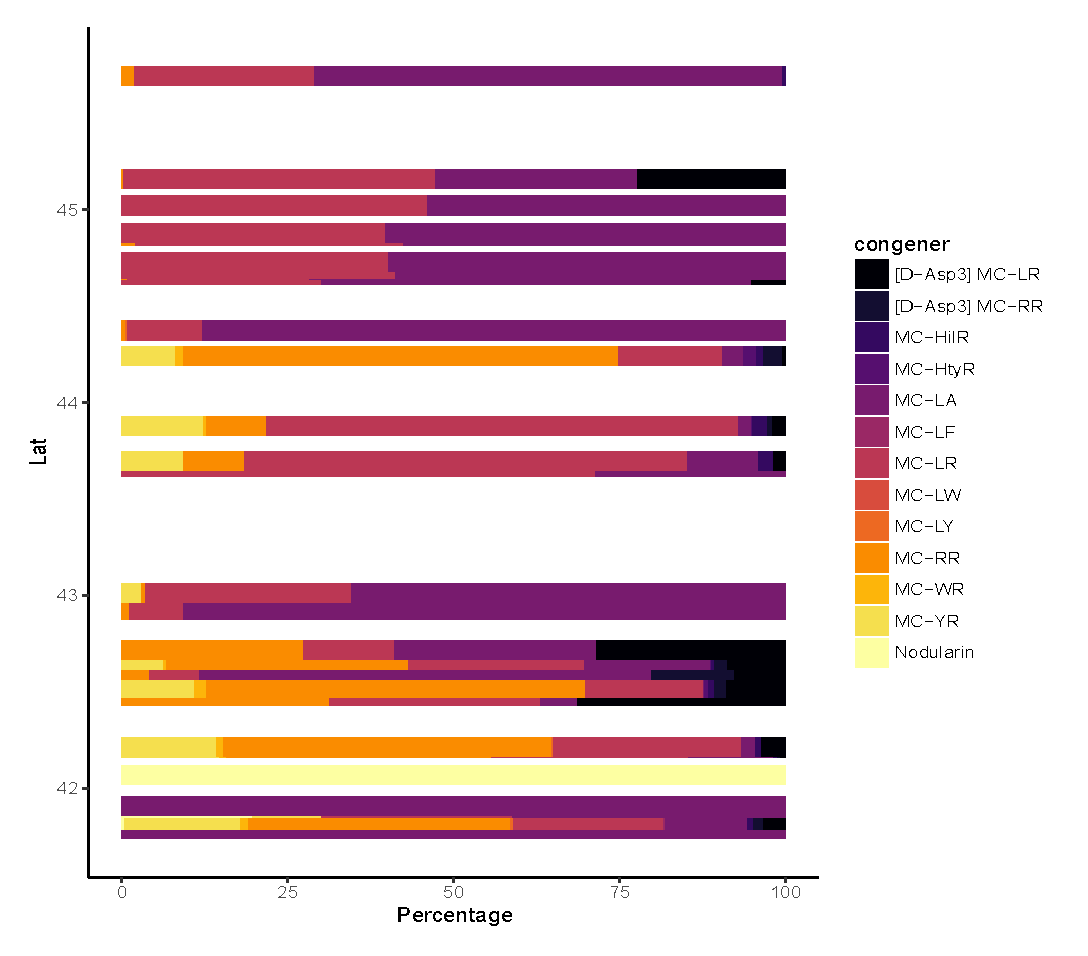
\includegraphics[scale=0.9]{congeners}
  \label{ss}
\end{figure}

\newpage

%congener plot
\begin{figure}[!htp]
  \caption{title}
  \includegraphics[scale=0.7]{congenerplot}
\end{figure}

\newpage

\begin{table}[!htbp]
  \centering
  \caption{Summary Statistics of MC from Grab Sample}
  \label{statsmc}
\begin{tabular}{@{\extracolsep{5pt}}lccccc}
\\[-1.8ex]\hline
\hline \\[-1.8ex]
Statistic & \multicolumn{1}{c}{N} & \multicolumn{1}{c}{Mean} & \multicolumn{1}{c}{St. Dev.} & \multicolumn{1}{c}{Min} & \multicolumn{1}{c}{Max} \\
\hline \\[-1.8ex]
Nodularin & 114 & 0.0003 & 0.002 & 0.030 & 0.021 \\
{[D-Asp3]}MC-RR & 114 & 0.006 & 0.028 & 0.030 & 0.255 \\
MC-RR & 114 & 0.185 & 0.855 & 0.030 & 8.552 \\
MC-YR & 114 & 0.046 & 0.202 & 0.030 & 1.799 \\
MC-HtyR & 114 & 0.002 & 0.012 & 0.030 & 0.107 \\
MC-LR & 114 & 0.142 & 0.447 & 0.030 & 3.570 \\
{[D-Asp3]}MC-LR & 114 & 0.027 & 0.107 & 0.030 & 0.902 \\
MC-HilR & 114 & 0.004 & 0.019 & 0.030 & 0.150 \\
MC-WR & 114 & 0.005 & 0.029 & 0.030 & 0.302 \\
MC-LA & 114 & 0.088 & 0.196 & 0.030 & 1.729 \\
MC-LY & 114 & 0.0004 & 0.002 & 0.030 & 0.024 \\
MC-LW & 114 & 0.030 & 0.030 & 0.030 & 0.030 \\
MC-LF & 114 & 0.0002 & 0.001 & 0.030 & 0.012 \\
MC Sum from LC MS/MS  & 114 & 0.505 & 1.580 & 0.000 & 14.857 \\
MC from ELISA & 115 & 0.747 & 1.784 & 0.030 & 15.320 \\
\hline \\[-1.8ex]
\multicolumn{6}{r}{Values are expressed as($\mu$g of MC*${L^{-1}}$)} \\
\end{tabular}
\end{table}

 \newpage

\appendixchapter{SPATTs}

Solid Phase Adsorption Toxin Tracking (SPATTs) is a novel method of monitoring waterbodies. A Nitex mesh bag containing HP-20 resin (styrene-divinylbenzene copolymer) is submerged in waterbody of interest for a period of time. During this period, free-floating compounds will adsorb onto the polymer beads. SPATTs can are then retrieved and analyzed for chemical analytes of interest. This technique can be useful if sampling frequency is financially limited.

\section*{Methods}

\subsection*{Construction of SPATTs}

A 1 meter x 5 centimeter strip of Nitex mesh were precisionaly cut. The Nitex strip was sewn by folding half lenth-wise (or \emph{hot dog} style). With tape holding the fold, the end of the strip was sewn 0.5cm from the edge. Stiching design was tight to ensure no leakage of polymer beads.

9-10cm of sewn Nitex strips were cut and zip-tied about 0.5cm at one end. 3.00-3.01 grams of HP-20 resin was filled using a funnel. The other end is zip-tied once the Nitex bag is full. SPATT bags are activated by soaking in 100\% methanol for 24 hours under $4^\circ$C. Next the SPATTs were rinsed with Milli-Q water and then soaked for 24 hours in Milli-Q water under $4^\circ$C.



\subsection*{Deployment}


\appendixchapter{Statistical Analysis}

\appendixchapter{Data Collection Guide}

\section*{Purpose}


\indent I explored with the tool from Open Data Kit \footnote{Open Data Kit 2.0: Expanding and Refining Information Services for Developing Regions \url{http://www.hotmobile.org/2013/papers/full/2.pdf} Waylon Brunette, Mitchell Sundt, Nicola Dell, Rohit Chaudhri, Nathan Breit, Gaetano Borriello In HotMobile, 2013. \url{http://dl.acm.org/citation.cfm?id=2444790}} and has served me in other projects with limited resources  in great sucess. I discovered a way to create a centralized database and had my teammates collect data using their smart phone. With the limited time on my hand, I accomplished my task with ease. I could not have done it without these tools. The alternative would be laborious, involving me to compile multiple data. Doing so does increases the posibility of error from copy and pasting data into an organized datasheet.
With this experience, I wish to help other research studies with a cheaper alternative and greatly facilitate their pursuit. I have written this guide in building from the ground up on setting a database and providing a viable way to organize an enterprise. This guide is aimed for non-profit organization and academic research with a limited budget. The cost is merely \$5 per month for a virtual private server or free if one chooses to host their own machine server.

\section*{Data Collection}


\indent Large scale studies are often done by a team of multiple groups and organiziations. Data aggregation and structural collection is one of the few key factors that determines the quality of the study.

\section*{Server Setup}

\indent Here we must setup a server that stores our data and be accessible through the internet. Having your own computer machine as a server is a viable solution but it requires more extensive networking knowledge. An alternative solution is to purchase a rent a server from a third party which automatically sets up and quickly gets connected to the internet.

A Virtual Private Server (VPS) are cheap and flexible servers to set up a database up on the cloud. For as little as \$5 dollars a month one can have a server with everything they need to start collecting data.

DigitalOcean, Amazon (free trial for a year), Google VPS can work. I suggest anyone of them, but in this guide we will choose to setup from DigitalOcean as its the cheapest available. I reccomend Debian or Ubuntu linux distro to setup our database. here we will choose Debian 9 (Stretch).

Use your SSH client. For Linux or Mac, use terminal. Windows could use putty. Access your server by SSH. You need to know what the IP address is for your server, the user name and password. Usually this is emailed to you from the providor.

\noindent The command for terminal is

\begin{lstlisting}[language=bash]
  $ ssh root@xxx.xxx.xxx
\end{lstlisting}



\end{appendix}

\end{document}
